%%%%%%%%%%%%%%%%%%%%%%%%%%%%%%%%%%%%%%%%%
% University/School Laboratory Report
% LaTeX Template
% Version 3.1 (25/3/14)
%
% This template has been downloaded from:
% http://www.LaTeXTemplates.com
%
% Original author:
% Linux and Unix Users Group at Virginia Tech Wiki 
% (https://vtluug.org/wiki/Example_LaTeX_chem_lab_report)
%
% License:
% CC BY-NC-SA 3.0 (http://creativecommons.org/licenses/by-nc-sa/3.0/)
%
%%%%%%%%%%%%%%%%%%%%%%%%%%%%%%%%%%%%%%%%%

%----------------------------------------------------------------------------------------
%	PACKAGES AND DOCUMENT CONFIGURATIONS
%----------------------------------------------------------------------------------------

\documentclass{article}

\usepackage[version=3]{mhchem} % Package for chemical equation typesetting
\usepackage{siunitx} % Provides the \SI{}{} and \si{} command for typesetting SI units
\usepackage{graphicx} % Required for the inclusion of images
\usepackage{natbib} % Required to change bibliography style to APA
\usepackage{amsmath} % Required for some math elements 

\setlength\parindent{0pt} % Removes all indentation from paragraphs

\usepackage{hyperref}
\hypersetup{
    colorlinks=true,
    linkcolor=blue,
    filecolor=magenta,      
    urlcolor=blue,
}

\renewcommand{\labelenumi}{\alph{enumi}.} % Make numbering in the enumerate environment by letter rather than number (e.g. section 6)

%\usepackage{times} % Uncomment to use the Times New Roman font

%----------------------------------------------------------------------------------------
%	DOCUMENT INFORMATION
%----------------------------------------------------------------------------------------

\title{Visualizing COVID-19 Outbreaks at Long Term Care Facilities in Ontario \\ 
		\large A Proposal to integrate the Open Database of Buildings and the Open Database of Healthcare Facilities with COVID-19 data}


\author{Shreeram \textsc{Murali} \\ KT \textsc{Hobbs} \\ Ngan \textsc{Lyle} \\ Sofia \textsc{Bahmutsky}}

\date{\today} % Date for the report

\begin{document}

\maketitle % Insert the title, author and date

\begin{center}
\begin{tabular}{l r}
Partners: & Bruno St-Aubin \\ % Partner names
& Marian Radulescu \\
Instructor: & Scott Fazackerley % Instructor/supervisor
\end{tabular}
\end{center}

% If you wish to include an abstract, uncomment the lines below
% \begin{abstract}
% Abstract text
% \end{abstract}

%----------------------------------------------------------------------------------------
%	SECTION 1
%----------------------------------------------------------------------------------------

\section{Introduction}

Since its initial appearance in China on December 31, 2019, Coronavirus disease, or COVID-19, has evolved to a global pandemic --- a novel disease to which there is little pre-existing immunity that becomes epidemic in many countries. At the time of writing, COVID-19 has spread to more than 180 countries (1). Worldwide, there are greater than 3 million confirmed cases and greater than 230,000 deaths (2). In Canada, there have been almost 60,000 confirmed cases with almost 18,000 cases and 1,300 deaths in Ontario alone (3). As the pandemic spread, it has become clear that seniors shoulder a disproportionate burden of disease. In fact, almost half of fatalities in Canada are related to outbreaks among seniors in long term care facilities (4). This proposal seeks to integrate a number of open source Statistics Canada databases to provide insight into the COVID-19 outbreak among long term care facilities in Ontario. Our goal is to create an interactive visualization of long term care facilities in Ontario as well as an article exploring the spread of COVID-19 among long term care facilities in Canada. 



% If you have more than one objective, uncomment the below:
%\begin{description}
%\item[First Objective] \hfill \\
%Objective 1 text
%\item[Second Objective] \hfill \\
%Objective 2 text
%\end{description}

\section{Resources}
\label{Data}
We will be using the following open databases from the Linkable Open Data Environment (LODE):

\begin{description}

\item[Open Database for Health Facilities (ODHF) data]
A comma-separated file of health facility information across Canada with missing address information.

\item[Open Database of Buildings (ODB) data]
A spatial database of buildings across Canada. We will focus on data for Ontario.

\item[Proximity data for transit, health care, pharmacies (time permitting)]
A comma-separated file of proximity metrics across Canada on the regional level. We will focus on data for Ontario.

\end{description} 

In addition, we will be using the Ontario provincial health COVID data. 
 
  
%----------------------------------------------------------------------------------------
%	SECTION 2
%----------------------------------------------------------------------------------------

\section{Proposed Project}

\subsection{Objectives}

This project involves analyzing open source data and using interactive visualizations to produce an exploratory analysis tool for observing potential relationships within data. To build the required dataset, we will initially merge several sources: ODHF, ODB, proximity data, and COVID-19 data. Pursuits will focus on data for the province of Ontario. ODHF data will also require completing missing addresses, which we aim to accomplish by web scraping. Once the ODHF data is complete, it would be joined to ODB on location columns (latitude/longitude). Finally, proximity and COVID-19 datasets could also be joined on location columns.\\

Once data cleaning and integration is complete, it would be used to create interactive maps that depict location and severity of COVID-19 cases in senior care facilities in Ontario in addition to a time-lapse of the daily cases. Ideally, this would be accomplished using shape files from the ODB as well as GIS, and D3 to build a dashboard. \\

Finally, the created visualizations would be used for exploratory data analysis and observation of relationships within the data to gain insight about COVID-19 and the senior care facilities that are affected. Combined with proximity data, the visualizations could show connections between COVID-19 and other regional/spatial factors that may not have been considered previously. \\

There are two main objectives:

\begin{center}
\begin{itemize}
\item To ensure quality and possible improvement of the open data sources (ODHF and COVID-19).

\item To produce products showing that open data (including the databases that we are using from the LODE) are usable in complex analytical cases, resulting in high quality interactive visualizations and analyses.


\end{itemize}
\end{center}


\subsection{Deliverables}

\begin{center}
\begin{itemize}
\item Complete and clean ODHF dataset with a focus on senior care facilities in Ontario.

\item OBD with attributes linked to some building footprints, with a focus on healthcare facilities in Ontario.

\item Visualizations integrating healthcare facilities, proximity metrics and COVID-19 outbreak data in Ontario. 

\item Research paper that includes exploratory analysis of patterns and/or connection between ODB, ODHF, proximity data, and COVID-19 data.


\end{itemize}
\end{center}

\subsection{Schedule}

\begin{figure}[h]
\begin{center}
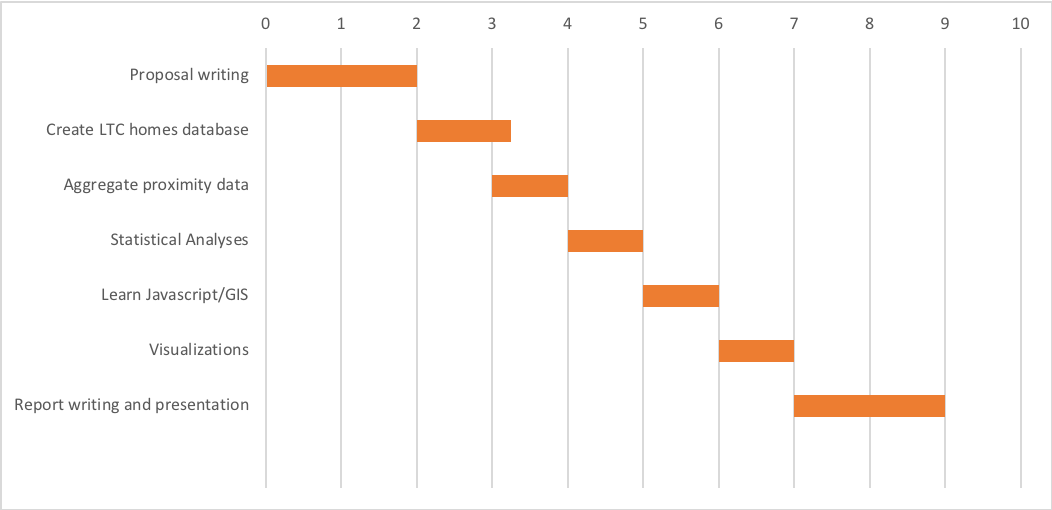
\includegraphics[width=0.65\textwidth]{schedule} % Include the image placeholder.png
\caption{Schedule for completion of tasks for the project in weeks.}
\end{center}
\end{figure}

\subsubsection{Schedule Details}
\begin{table}[h!]
	\begin{center}
   	 \caption{Details for Selected Tasks}
   	 \label{tab:table1}
		\begin{tabular}{l|p{105mm}}
			\textbf{Task} & \textbf{Details} \\
 			\hline\hline
 			Complete ODHF & \textbf{1.} Complete missing addresses \newline \textbf{2.}  Complete missing facility types\\
 			\hline
 			Clean ODHF & \textbf{1.}  Ensure data types and structures are compatible between sources \newline \textbf{2.} Resolve duplicate entries\\
 			\hline
			Merge Data & \textbf{1.} Merge ODHF with ODB \newline \textbf{2.} Merge with COVID-19 Ontario case data\\
			\hline
			Learn Javascript/GIS & Learn how to implement using D3\\
			\hline
			Visualizations & \textbf{1.} Interactive Choropleth Map of COVID-19 case numbers by health region in Ontario with time lapse \newline \textbf{2.} Interactive map of long term care facilities in Ontario with COVID-19 metadata\\

		\end{tabular}

	\end{center}
\end{table}



The project will begin as soon as permission is granted to proceed and will proceed according to the schedule shown in \textbf{Figure 1}. Details for selected tasks are shown in \textbf{Table 1}. The final report will be completed by the week of June 15th.


\subsection{Limitations}

The proposed project, including data preparation, analysis, visualization and report writing, is being undertaken on a compressed timeline and includes exposure to new tools and programming languages such as JavaScript and GIS. As a result, the deliverables will likely require assistance and further review before they are publishable.
 


\section{Bibliography}

\textbf{1} \href{https://www.arcgis.com/apps/opsdashboard/index.html#/bda7594740fd40299423467b48e9ecf6}{John Hopkin's COVID-19 Dashboard}\\

\textbf{2} \href{https://www.arcgis.com/apps/opsdashboard/index.html#/bda7594740fd40299423467b48e9ecf6}{WHO arcGIS Dashboard}\\

\textbf{3} \href{https://www.ontario.ca/page/how-ontario-is-responding-covid-19}{How Ontario is responding to COVID-19}\\

\textbf{4} \href{https://www.theglobeandmail.com/canada/article-outbreaks-at-seniors-homes-linked-to-almost-half-of-covid-19-deaths/}{Outbreaks at seniors’ homes linked to almost half of COVID-19 deaths in Canada, Theresa Tam says}\\

\textbf{5} \href{https://data.ontario.ca/dataset/confirmed-positive-cases-of-covid-19-in-ontario/resource/455fd63b-603d-4608-8216-7d8647f43350}{Confirmed positive cases of COVID-19 in Ontario}

%----------------------------------------------------------------------------------------
%	BIBLIOGRAPHY
%----------------------------------------------------------------------------------------
\bibliographystyle{unsrt}
\bibliography{refs.bib}



%----------------------------------------------------------------------------------------


\end{document}